\documentclass[25pt, a0paper, portrait]{tikzposter}

\usepackage[utf8]{inputenc}
\usepackage[T1]{fontenc}
\usepackage{lmodern}
\usepackage{graphicx}
\usepackage{amsmath}
\usepackage{booktabs}
\usepackage{enumitem}

\usetheme{Board}
\usecolorstyle{Default}
\useblockstyle{Default}
\colorlet{backgroundcolor}{white}
\tikzposterlogo{}

\title{\parbox{\linewidth}{\centering Lexical Functions to Improve Lexical Competence}}
\author{Na An$^1$, Gabriel Beaudoin$^2$, Noah Tremblay Taillon$^3$}
\institute{$^1$na.an1@umontreal.ca, $^2$gabriel.beaudoin.3@umontreal.ca, $^3$noah.tremblay.taillon@umontreal.ca\\ Université de Montréal}

\begin{document}

\maketitle

\begin{columns}

    \column{0.5}

    \block{1. Introduction \& Motivation}{
        \begin{itemize}[label=\textbullet, itemsep=10pt]
            \item \textbf{The Problem:} Large Language Models (LLMs) perform very well on general tasks, but their fine-grained understanding of semantic and lexical relations remains limited compared to human native speakers.
            \item \textbf{Proposed Solution:} Utilize the Meaning-Text Theory (MTT) and its \textbf{Lexical Functions (LFs)} to structurally inject lexical knowledge into models.
            \item \textbf{Objective:} Evaluate whether explicit fine-tuning on a structured dataset improves both specific lexical competence and general Natural Language Understanding (NLU).
        \end{itemize}
    }

    \block{2. Methodology}{
        \begin{itemize}[label=\textbullet, itemsep=10pt]
            \item \textbf{Dataset:} Data extracted from the \textit{French Lexical Network (fr-LN)}, formatted in JSON (POS, senses, LFs, in-context examples). 80\% train / 20\% test split.
            \item \textbf{Evaluated Models:} 
            \begin{itemize}
                \item \textbf{Mistral-7B} (Modern, multilingual)
                \item \textbf{Qwen2.5-7B} (Instruction-tuned, multilingual)
                \item \textbf{FlauBERT} (French-specific, Masked Language Model)
            \end{itemize}
            \item \textbf{Approach:} Parameter-Efficient Fine-Tuning (\textbf{LoRA}) to inject MTT constraints without prohibitive computational costs ($r=16, \alpha=32$).
            \item \textbf{Baselines:} Base \textit{un-finetuned} models and models fine-tuned on unstructured \textit{Wikipedia} text (to isolate the impact of MTT structure versus mere exposure to the French language).
        \end{itemize}
    }

    \block{3. COLE Benchmark}{
        \begin{center}
            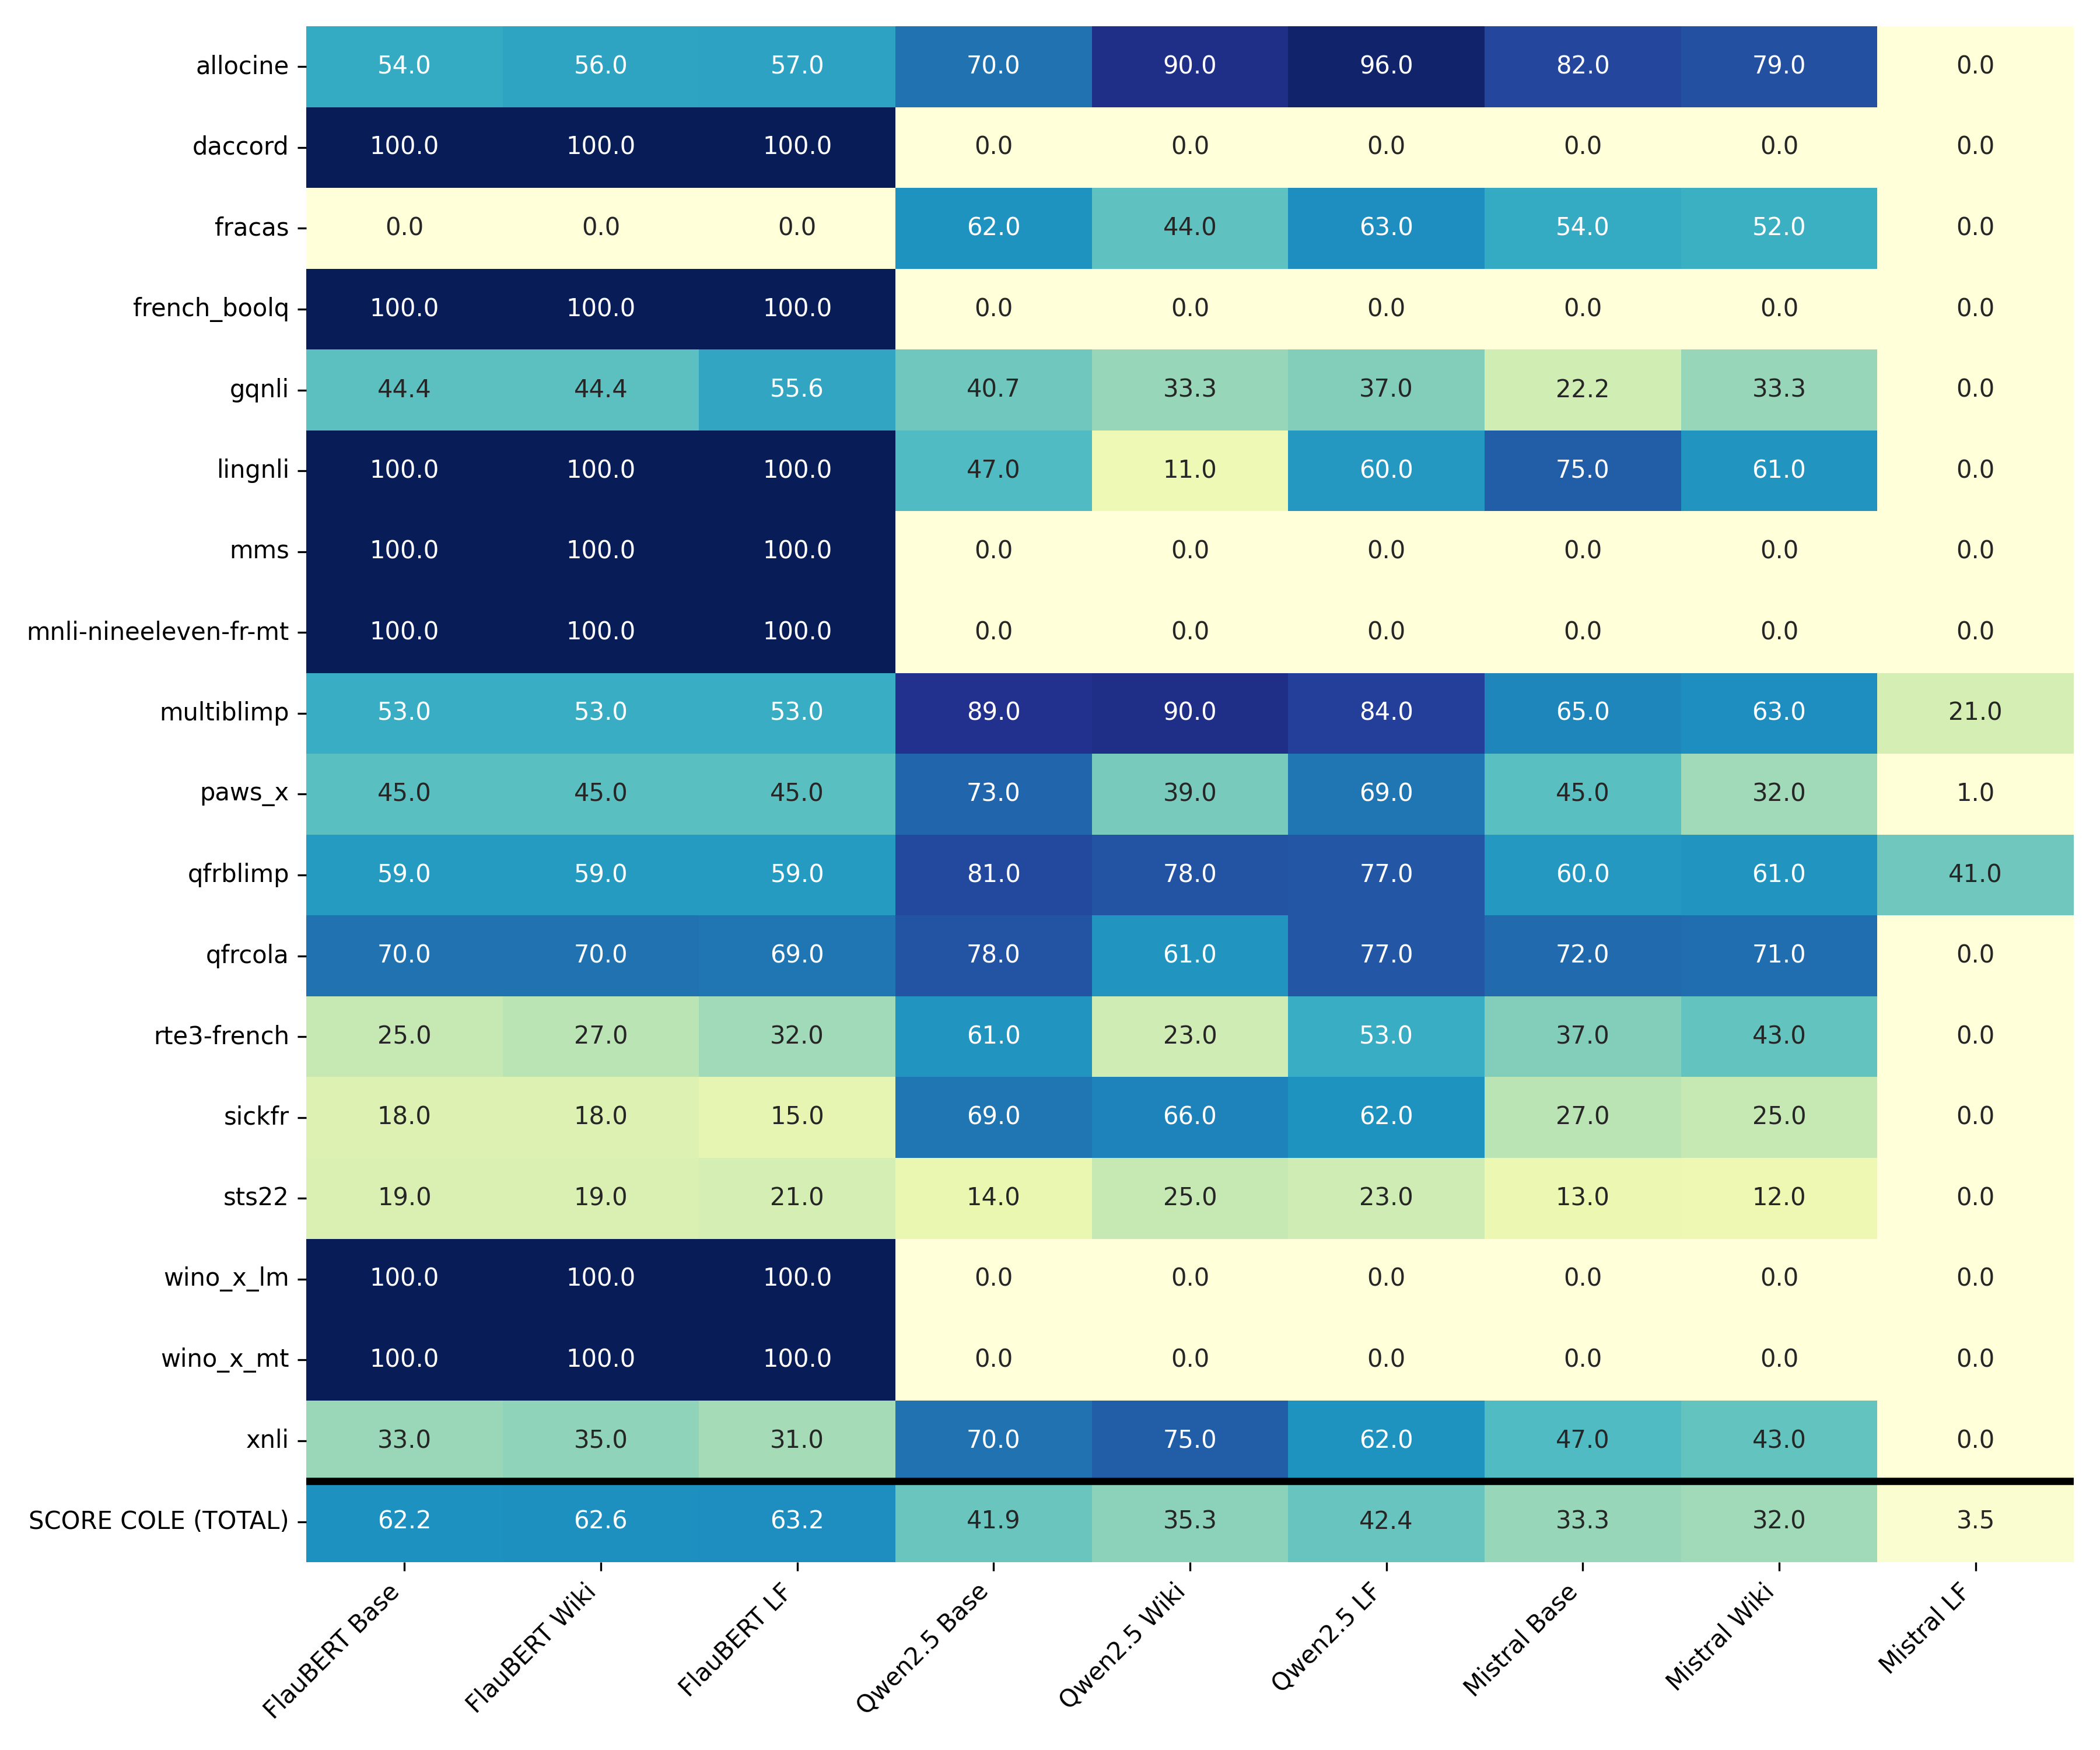
\includegraphics[width=0.95\linewidth]{figures/cole_heatmap.png}
        \end{center}
        \vspace{1cm}
        \textbf{Key Observations:}
        \begin{itemize}[label=\textbullet, itemsep=8pt]
            \item \textbf{Evaluation Format Mismatch:} Encoders (FlauBERT) naturally excel at COLE's exact classification tasks, while decoders (Qwen/Mistral) often fail artificially (scoring 0.0\%) due to strict expected-token constraints rather than true capability deficits.
            \item \textbf{Catastrophic Forgetting in Mistral:} Mistral LF's score collapsed to 3.5\%, scoring 0.0\% on almost all tasks, proving it overlearned the LF structure at the expense of general language modeling.
            \item \textbf{Minor General Gains:} Qwen LF showed slight NLU improvements over its base model, while FlauBERT's scores remained mostly stable across configurations.
        \end{itemize}
    }

    \column{0.5}

    \block{4. LF Benchmark}{
        \begin{center}
            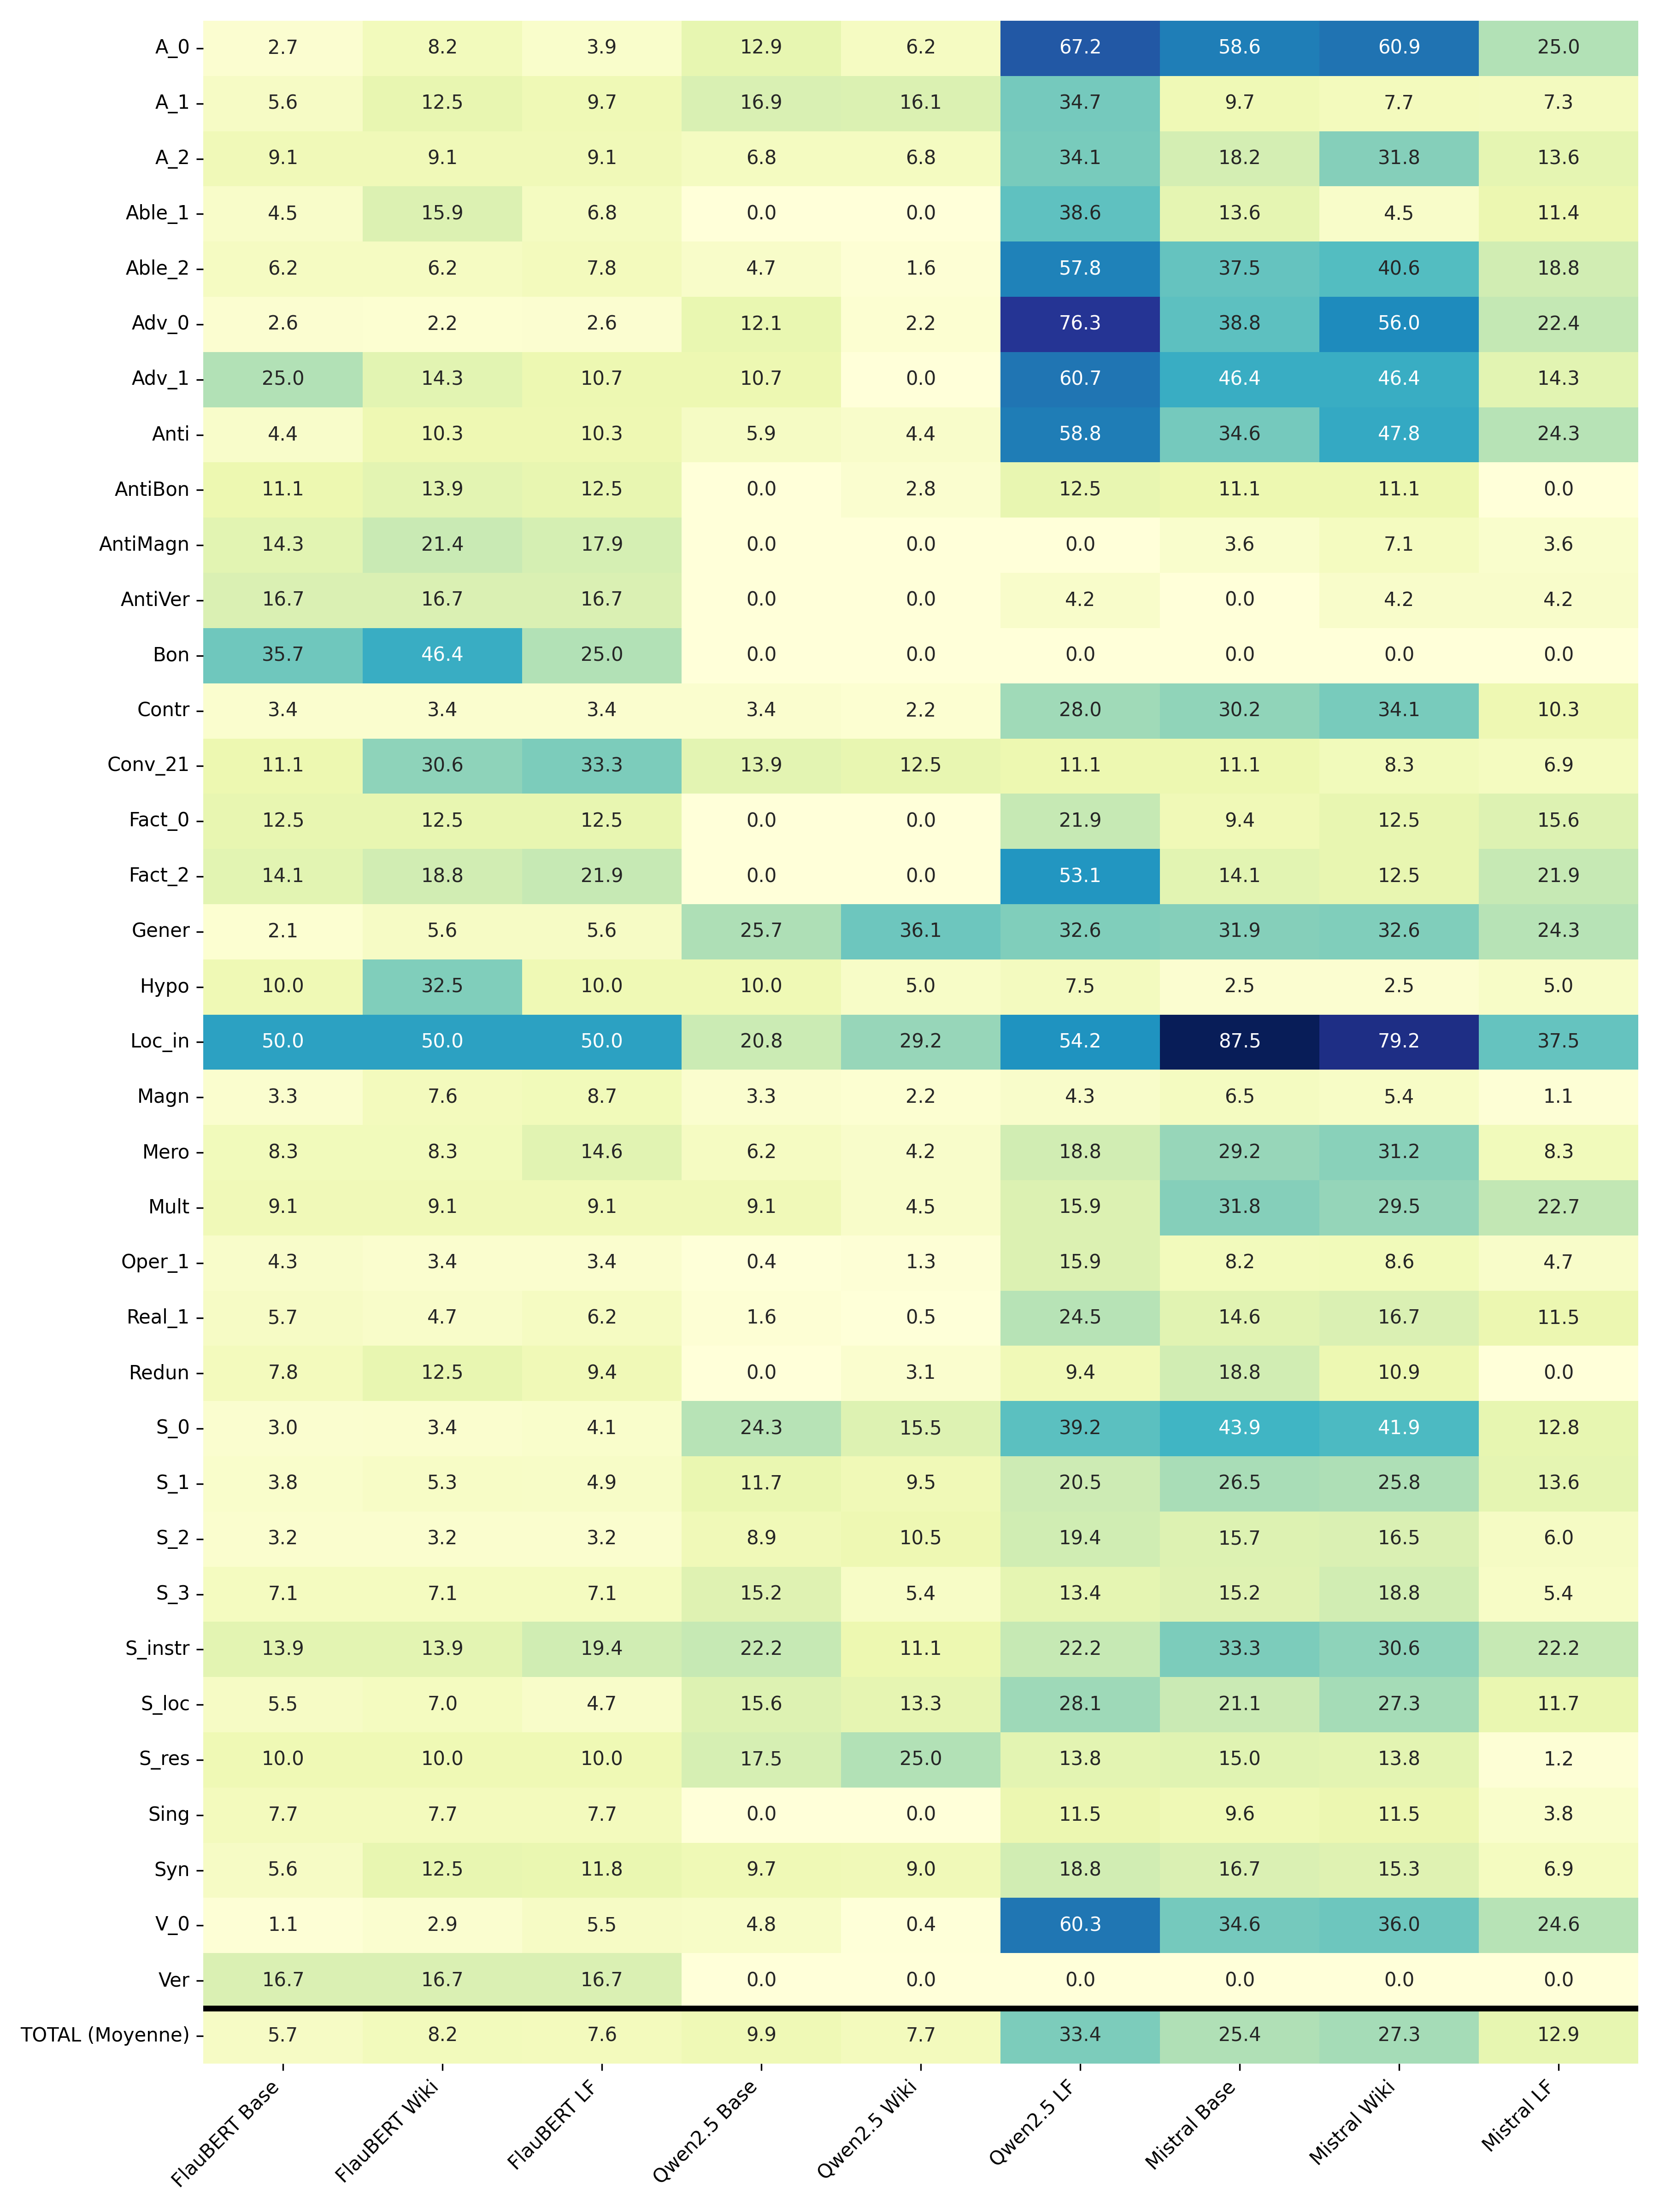
\includegraphics[width=0.95\linewidth]{figures/fl_heatmap.png}
        \end{center}
        \vspace{1cm}
        \textbf{Key Observations:}
        \begin{itemize}[label=\textbullet, itemsep=8pt]
            \item \textbf{Qwen2.5's Breakthrough:} Fine-tuning more than tripled its score (9.9\% $\rightarrow$ 33.4\%). It learned to respect the strict single-lexeme constraints, excelling in POS-change functions.
            \item \textbf{Mistral's Overfitting:} Base model performed well (25.4\%), but fine-tuning caused a severe performance drop (to 12.9\%), indicating catastrophic forgetting of its initial linguistic priors.
            \item \textbf{FlauBERT's Stagnation:} Scores remained stable but low (5.7\% $\rightarrow$ 8.2\%), likely due to an insufficient learning rate causing a ceiling effect for meaningful parametric shifts.
            \item \textbf{Structure Matters:} Fine-tuning on unstructured Wikipedia data did not consistently beat base models, confirming that raw text exposure does not substitute for explicit structured annotations.
            \item \textbf{Universal Gaps:} Relations like \textit{Ver, AntiVer,} and \textit{Bon} proved universally difficult, suggesting severe data scarcity in models' pre-training corpora.
        \end{itemize}
    }

    \block{5. Conclusion}{
        \textbf{Mixed and Architecture-Dependent Results:}
        \begin{itemize}[label=\textbullet, itemsep=10pt]
            \item \textbf{The Success:} Structural injection works: it more than tripled Qwen2.5's performance on understanding specialized lexical functions.
            \item \textbf{The Caveat:} Improving specific lexical competence does not smoothly translate into broader general NLU improvements (as seen on the COLE benchmark).
        \end{itemize}
        
        \vspace{1cm}
        {\LARGE \textbf{Future Work}}
        \vspace{0.5cm}
        
        Future research should explore alternative integration methods that are less prone to catastrophic forgetting: Soft-prompting, dynamically adapting LoRA hyperparameters, or integrating LF data directly during the standard alignment phases (RLHF/DPO) to balance specialized knowledge and robust general linguistic capabilities.
    }

\end{columns}

\end{document}